For ideal Lissajous curves, the paramaterization is also a path in $\R^2$. As a result, we can take path integrals. We essentially did this to find the arc length. The equation for a path integral is: \[\oint_{C}f(\vec{c}(t))\|\vec{c}^{\ \prime}(t)\|dt\] When calculating the arc length we had essentially set $f(\vec{c}(t)) = 1$. Which creates a path integral where the height at every point is equal to $1$, and thus the final value is the same as the arc length. However, we aren't limited to solely finding the arc length. For example, we could take a path integral over any function $f(x,y)$. I provide an example below:
\begin{center}
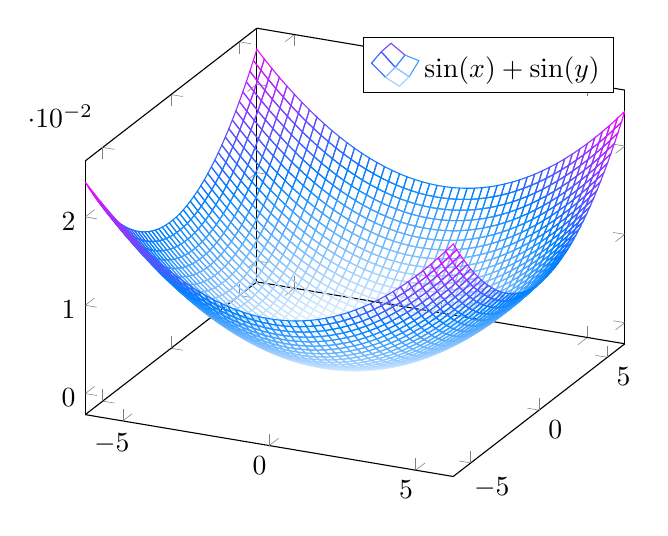
\begin{tikzpicture}[scale=1][h]
\begin{axis}[
    colormap/cool,
]
\addplot3[
    mesh,
    samples=50,
    domain=-2*pi:2*pi,
]
{sin(x)^2+sin(y)^2};
\addlegendentry{$\sin(x)+\sin(y)$}
\end{axis}
\end{tikzpicture}
\end{center}
